% "{'classe':('PSI'),'chapitre':'slci_revisions','type':('td'),'titre':'Robot à câbles', 'source':'Concours Centrale-Supélec 2023 - TSI','comp':(None),'corrige':True}"
%\setchapterimage{bandeau}
\chapter*{TD \arabic{cptTD} \\ 
Robot à câbles -- 
\ifprof Corrigé \else Sujet \fi}
\addcontentsline{toc}{section}{TD \arabic{cptTD} :
Robot à câbles -- 
\ifprof Corrigé \else Sujet \fi}

\iflivret \stepcounter{cptTD} \else
\ifprof  \stepcounter{cptTD} \else \fi
\fi

\setcounter{question}{0}
\marginnote{Concours Centrale-Supélec 2023 -- TSI.}
%\marginnote[1cm]{
%\UPSTIcompetence[2]{C1-02}
%\UPSTIcompetence[2]{C2-04}}

\begin{marginfigure}
\centering
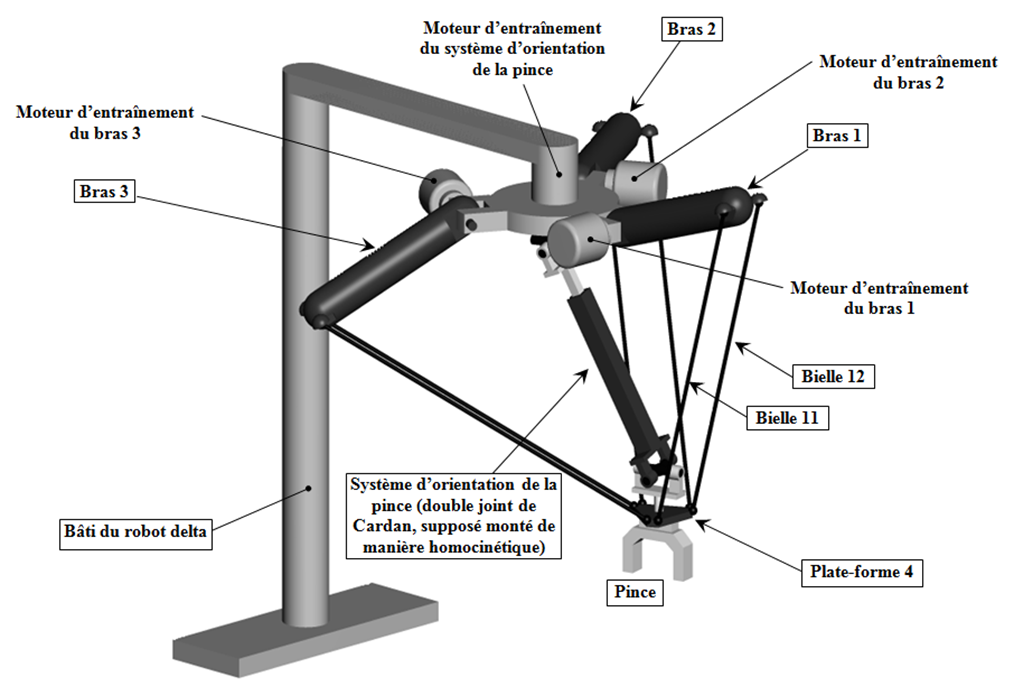
\includegraphics[width=\linewidth]{fig_01}
\caption{Robot à câbles CAROCA \label{Cy_02_Ch_04_TD_01_fig_01}}
\end{marginfigure}


\subsection*{Présentation}
\ifprof
\else
 Les robots parallèles à câbles sont une structure de robots apparus au début des années 2000. Dans ce système, la plate-forme est déplacée et orientée par rapport à une référence fixe dans toutes les directions de l’espace par l’enroulement ou le déroulement de plusieurs câbles (figure \ref{Cy_02_Ch_04_TD_01_fig_01}). Cette structure permet à la plate-forme d’atteindre une grande zone de travail avec une très grande précision dans le positionnement comme dans l’orientation.

% Les performances attendues pour ce robot à câbles sont précisées dans le tableau \ref{Cy_02_Ch_04_TD_01_tab_01}.
%
%\begin{table}[!h]
%\centering
%\begin{tabular}{llp{5.5cm}}
%\hline
%\textbf{Exigences} & \textbf{Niveau} & \textbf{Remarques} \\
%\hline
%Charge déplacée & $\leq \SI{616}{kg}$ & Valeur limitée par la résistance des câbles \\
%Précision de positionnement & $\leq \SI{10}{mm}$ & Dans les trois directions de l’espace \\
%Vitesse de translation & $\leq \SI{1}{m.s^{-1}}$ & Selon les trois directions de l’espace \\
%Accélération de translation & $\leq  \SI{0,5}{m.s^{-2}}$ & Selon les trois directions de l’espace \\
%\hline
%\end{tabular}
%\caption{Performances attendues pour le robot à câbles au niveau de la plate-forme suspendue \label{Cy_02_Ch_04_TD_01_tab_01}}
%\end{table}
\fi

\subsection*{Étude de l’asservissement de la longueur d’un câble pour gérer le mouvement}
%\noindent\begin{minipage}[c]{.6\linewidth}

\begin{obj}
Déterminer les réglages de la commande asservie des moteurs permettant d’assurer l’enroulement
 adéquat des câbles.
\end{obj}

\ifprof
\else
Le programme de pilotage tient compte de l’allongement relatif des câbles suite aux efforts de traction lors du déplacement de la plate-forme chargée. Il génère alors, pour chacun des huit moteurs, des consignes de position et de vitesse qui sont envoyées aux variateurs de vitesse qui alimentent les moteurs afin d’assurer un positionnement de la plate-forme conforme aux attentes de l’utilisateur.
L’ensemble composé d’un variateur et du moteur associé est appelé moto-variateur pour la suite. L’algorithme implanté dans le variateur est de type commande vectorielle, ce qui rend le moto-variateur équivalent à un  système du premier ordre avec une bande passante à $-\SI{3}{dB}$ de $\SI{200}{Hz}$.
 Le modèle défini figure \label{Cy_02_Ch_04_TD_01_fig_11} est adopté pour la suite.
 
 \begin{figure} [!h]
\centering
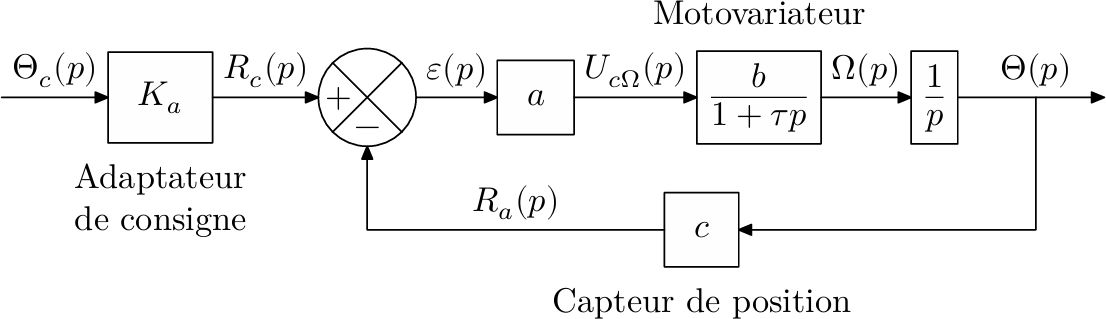
\includegraphics[width=.8\linewidth]{fig_11}
\caption{Schéma-bloc de la commande en position du moteur \label{Cy_02_Ch_04_TD_01_fig_11}}
\end{figure}

\subsection*{Notations}

\begin{itemize}
\item $\Theta_c(p)$ et $\Theta(p)$ sont respectivement les images de la consigne de position angulaire $\theta_c(t)$ (en rad) issue du programme de pilotage et de la position angulaire effective $\theta(t)$ du moteur (en \si{rad}). $\Omega(p)$ est l’image de la vitesse angulaire $\omega(t)=\thetap(p)$ du moteur (grandeur temporelle en \si{rad.s^{-1}}).
 \item Le capteur de position (codeur optique incrémental associé à une unité de comptage sur 13 bits) est de gain $c=\SI{1304}{point.rad^{-1}}$.
 \item L’adaptateur est de gain $K_a$, grandeur en \si{point.rad^{-1}}.
  \item Le correcteur est de type proportionnel de gain $a$, ce qui permet de délivrer une tension $u_{c\Omega}(t)$ proportionnelle à l’écart $\varepsilon(t)$. Un pré-réglage a permis de choisir la valeur $a=\SI{43,4}{mV.point^{-1}}$.
\item Le comportement du motovariateur est assimilé à un premier ordre de gain $b=\SI{31,4}{rad.s^{-1}.V^{-1}}$ et de constante de temps $\tau = \SI{796}{\mu s}$.
\end{itemize}
\fi


\question{Justifier la valeur numérique proposée pour la constante de temps $\tau$.}
\ifprof
\begin{corrige}
Si la bande passant à $-\SI{3}{dB}$ est de $\SI{200}{Hz}$, on a une pulsation de cassure à \SI{200}{Hz} soit $\omega_{\tau}=\dfrac{1}{\tau} = 2\times \pi \times 200$ et $\tau = 7,9\times 10^{-4}= \SI{796}{\mu s}$.
\end{corrige}
\else
\fi

\ifprof
\else
Dans la structure de l’asservissement de position de la figure \ref{Cy_02_Ch_04_TD_01_fig_11}, l’erreur est définie par$\mu(t)=\theta_c(t) - \theta(t)$ (grandeur en rad) et l’écart par $\varepsilon(t) = r_c(t)-r_a(t)$(grandeur en point).
\fi

\question{On souhaite que l’erreur $\mu(t)$ soit nulle quand l’écart $\varepsilon(t)$ l’est : en déduire la relation entre $K_a$ et $c$.}
\ifprof
\begin{corrige}
Dans les conditions citées ci-dessus, il faut donc nécessairement $K_a = c$. 
\end{corrige}
\else
\fi

\question{Après avoir donné l’expression de la fonction de transfert en boucle ouverte $\indice{H}{bo}\left(j\omega\right)$, tracer son diagramme asymptotique de Bode (courbes de gain et de phase en précisant la valeur de la cassure et le gain associé) et esquisser le plus précisément possible l’allure des courbes réelles de réponse fréquentielle.}
\ifprof
\begin{corrige}
Par définition, $\indice{H}{bo}\left(j\omega\right) = \dfrac{abc}{p\left(1+\tau p\right)}$ avec $abc = 1304\times 31,4 \times \num{43,3e-3} = \SI{1773}{s^{-1}}$.


\begin{center}
\begin{tikzpicture}[xscale=15/6]
\tikzset{
semilog lines/.style={thin, bleuxp}, 
semilog lines 2/.style={semilog lines,bleuxpc},
semilog half lines/.style={semilog lines 2,dotted },
semilog label x/.style={semilog lines,below,font=\tiny,black},
semilog label y/.style={semilog lines,right,font=\tiny,black}
}
\begin{scope}[yscale=3/140]
\OrdBode{20}
\semilog{1}{5}{-100}{60}
\BodeAmp[orangexp,thin,samples=150]{1:5}{\POAmpAsymp{1773}{0.000794}+\IntAmp{1}}
\BodeAmp[orangexp,ultra thick,samples=150]{1:5}{\POAmp{1773}{0.000794}+\IntAmp{1}}

%\draw (-1.5,28) node {\footnotesize $20\log K$};
%\draw (1.1,10) node {\footnotesize $-$40 dB/d\'ecade};
%\draw [dashed,ultra thick,bleuxp] (-.08,-60) -- (-.08,25);
%\draw (-.08,-60)  node {\Huge $\cdot$} node [above right]{\footnotesize $\omega_0$};
\end{scope}
\begin{scope}[yshift=-3cm,yscale=1/90]
\UniteDegre
\OrdBode{45}
\semilog{1}{5}{-180}{0}
%\BodeArg[orangexp,thin,samples=150]{1:5}{\POArgAsymp{1773}{0.000794}+\IntAmp{1}}
\BodeArg[orangexp,thin,samples=150]{1:5}{\POArgAsymp{1773}{0.000794}+\IntArg{1}}
\BodeArg[orangexp,ultra thick,samples=190]{1:5}{\POArg{1773}{0.000794}+\IntArg{1}}

%\BodeArg[orangexp,samples=100,thin]{-2:2}{\SOArg{10}{0.2}{.9}}
%\BodeArg[orangexp,ultra thick]{-2:2}{\SOArg{10}{0.2}{.9}}
\end{scope}
\end{tikzpicture}
\end{center}


\end{corrige}
\else

\begin{center}
\begin{tikzpicture}[xscale=15/6]
\tikzset{
semilog lines/.style={thin, bleuxp}, 
semilog lines 2/.style={semilog lines,bleuxpc},
semilog half lines/.style={semilog lines 2,dotted },
semilog label x/.style={semilog lines,below,font=\tiny,black},
semilog label y/.style={semilog lines,right,font=\tiny,black}
}
\begin{scope}[yscale=3/140]
\OrdBode{20}
\semilog{1}{5}{-100}{60}
%\BodeAmp[orangexp,thin,samples=150]{1:5}{\POAmpAsymp{1773}{0.000794}+\IntAmp{1}}
%\BodeAmp[orangexp,ultra thick,samples=150]{1:5}{\POAmp{1773}{0.000794}+\IntAmp{1}}

%\draw (-1.5,28) node {\footnotesize $20\log K$};
%\draw (1.1,10) node {\footnotesize $-$40 dB/d\'ecade};
%\draw [dashed,ultra thick,bleuxp] (-.08,-60) -- (-.08,25);
%\draw (-.08,-60)  node {\Huge $\cdot$} node [above right]{\footnotesize $\omega_0$};
\end{scope}
\begin{scope}[yshift=-3cm,yscale=1/90]
\UniteDegre
\OrdBode{45}
\semilog{1}{5}{-180}{0}
%\BodeArg[orangexp,thin,samples=150]{1:5}{\POArgAsymp{1773}{0.000794}+\IntAmp{1}}
%\BodeArg[orangexp,thin,samples=150]{1:5}{\POArgAsymp{1773}{0.000794}+\IntArg{1}}
%\BodeArg[orangexp,ultra thick,samples=190]{1:5}{\POArg{1773}{0.000794}+\IntArg{1}}

%\BodeArg[orangexp,samples=100,thin]{-2:2}{\SOArg{10}{0.2}{.9}}
%\BodeArg[orangexp,ultra thick]{-2:2}{\SOArg{10}{0.2}{.9}}
\end{scope}
\end{tikzpicture}
\end{center}
\fi

\question{Relever sur la courbe tracée à la question précédente la valeur de la marge de phase $M\varphi$. Sachant  qu’on souhaite que cette marge soit de $M\varphi = 45\degres$, conclure quant au réglage de $a$.}
\ifprof
\begin{corrige}
La marge de phase est mesurée à enivron 45\degres. Le choix de $a$ est donc convenable. 
\end{corrige}
\else
\fi



\question{Déterminer l’expression de l’image $\mu(p)$ de l’erreur en fonction de l’image $\Theta_c(p)$ de la consigne angulaire  et de la fonction de transfert en boucle ouverte $\indice{H}{bo}(p)$ de l’asservissement.}
\ifprof
\begin{corrige}
Pour déterminer l'erreur vis-à-vis de la consigne, il faudrait déplacer le comparateur vers la gauche. Cela revient à avoir un asservissement à retour unitaire en passant le gain $c$ dans la chaîne directe. 

On a donc $\mu(p)=\dfrac{\Theta_c(p)}{1+FTBO(p)}$ avec $FTBO(p) = \dfrac{abc}{p\left(1+\tau p\right)}$.


Remarque : on peut aussi exprimer $\varepsilon(p) = \dfrac{R_c(p)}{1+FTBO(p)} =\dfrac{\Theta_c(p) a}{1+FTBO(p)}$. On a donc $\varepsilon(p) =a \mu(p)$.
\end{corrige}
\else
\fi


\ifprof
\else

\ifprof
\else
\marginnote{
\begin{solution}
\begin{enumerate}
\item . 
\item $K_a = c$.
\item $\indice{H}{BO}(j\omega)=\dfrac{1777}{j\omega\left(1+\dfrac{j\omega}{1256}\right)}$.
\item .
\item $\mu(p)=\dfrac{\Theta_c(p)}{1+\indice{H}{BO}(p)}$.
\item $\mu_p = 0$, $\mu_v = \dfrac{\omega_0}{abc}$.
\end{enumerate}
\end{solution}}
\fi

 La précision du système s’évalue par l’erreur en régime permanent pour des consignes de position de types :
 \begin{itemize}
 \item échelon d’amplitude $\theta_0$ (en \si{rad}) : l’erreur en régime permanent, notée $\mu_p$ (en rad), est dite « statique » ;
\item rampe de pente $\omega_0$ (en \si{rad.s^{-1}}) : l’erreur en régime permanent, notée $\mu_v$ (en \si{rad.s^{-1}}), est dite « de poursuite ».
\end{itemize}
Les exigences de l’utilisateur imposent que ces deux erreurs doivent être inférieures à 0,1\% de la consigne.
\fi

\question{Déterminer la valeur de l’erreur statique $\mu_p$. Déterminer l’expression de l’erreur de poursuite $\mu_v$ en fonction des gains $a$, $b$ et $c$ et de la pente $\omega_0$. Faire l’application numérique et vérifier si les exigences de l’utilisateur sont vérifiées.}
\ifprof
\begin{corrige}
La FTBO est de classe 1 et il n'y a pas de perturbation. On a donc $\mu_p = 0 $ et $\mu_v = \dfrac{\omega_0}{abc}$. Pour $\omega_0 =1$, on a $\mu_v =0,05\%$.
Le cahier des charges est respecté.
\end{corrige}
\else
\fi

 \begin{figure} [!h]
\centering
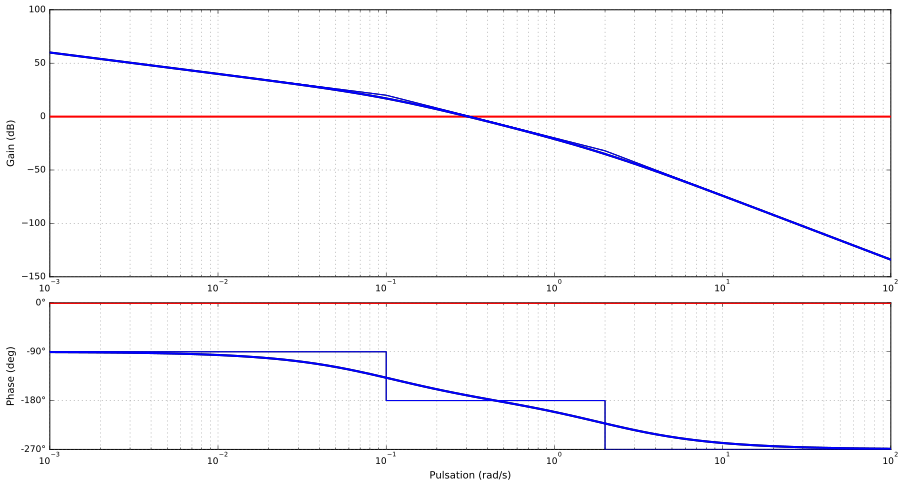
\includegraphics[width=.8\linewidth]{fig_03}
%\caption{Schéma-bloc de la commande en position du moteur \label{Cy_02_Ch_04_TD_01_fig_11}}
\end{figure}

